\documentclass[../master/master.tex]{subfiles}
\begin{document}
\todo[inline]{add missing data points for algorithms that timed out}
\todo[inline]{Add a comparison that shows the gain in time/step when restricting in lockstep - graph with lockstep and lockstepER showing time/symbollic step on y-axis with node counts on x-axis.}
This section describes the inputs we used for experiments, as well as the general observations made based on the results. To test and experiment with our implementation, we found datasets of different types and sizes. There are graphs with amount of nodes between 200 and 720000. The graphs also vary in the amount of SCCs which they contain, as we have some with as as little as 1 SCC and some with up to 25 thousand.

We have tested our implementations of the linear-time and Lockstep algorithms as descried in the papers \cite{linear}\cite{lockstep}, as well as our modification of the two using trimming and of lockstep using edge restriction. The data can be seen in Figure \ref{fig:data}

\subsection{Nodes vs. Steps}
We started by comparing the symbolic steps and number of nodes in the graph to the number of nodes, as the complexity of the algorithms was described in terms of these two. The two graphs below show that there is a somewhat positive correlation between number fo nodes and symbolic steps, with some outliers. 

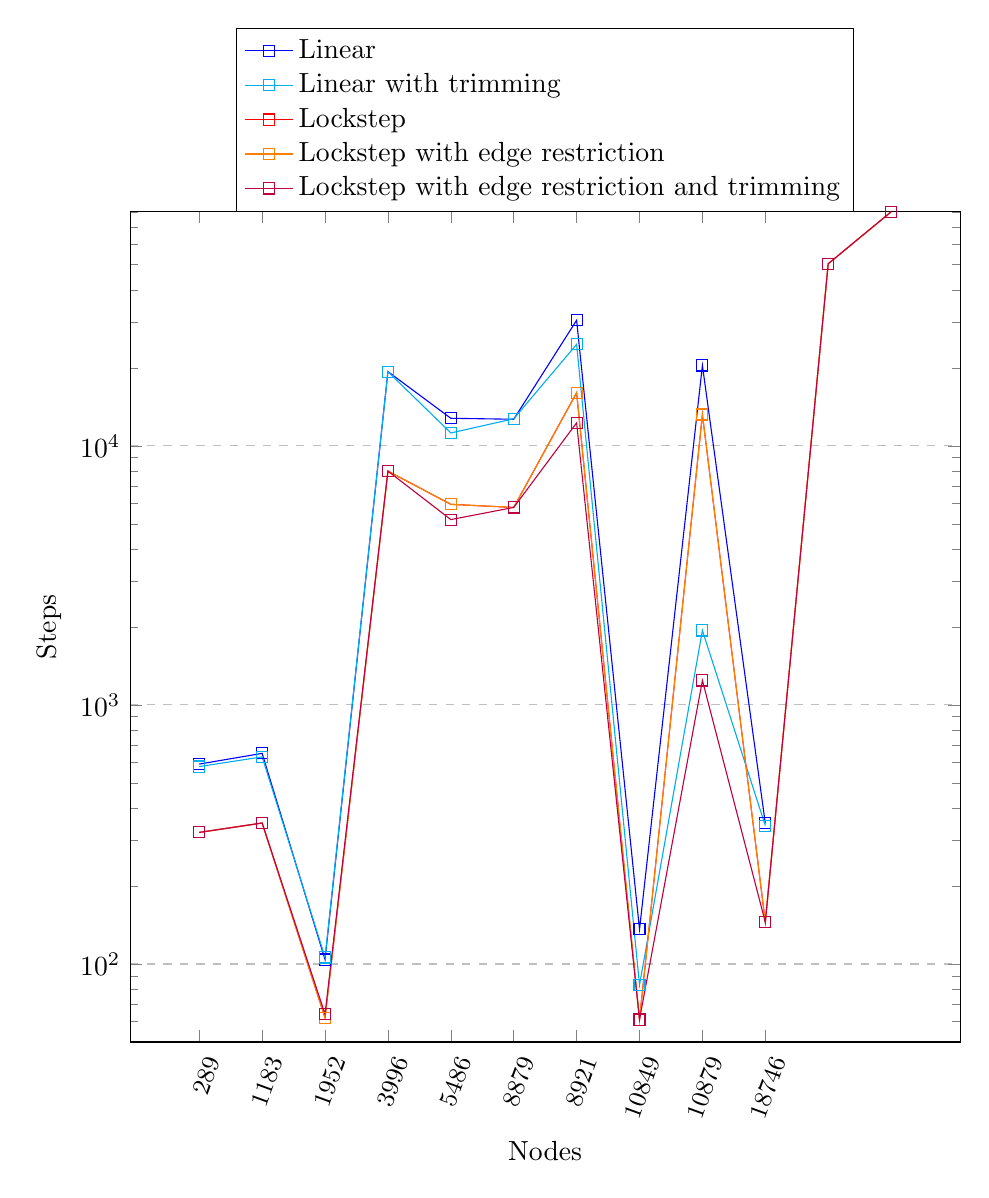
\begin{tikzpicture}
\begin{axis}[
height = \textwidth,
width=\textwidth,
xtick=data,
x tick label style = {font = \small, align = center, rotate = 70, anchor = north east},
title={Small graphs},
xlabel={Nodes},
ylabel={Steps},
ymin=50, ymax=80100,
legend style={at={(0.5,1)},anchor=south,legend cell align=left},
ymajorgrids=true,
grid style=dashed,
ymode=log,
log basis y={10},
symbolic x coords={289, 1183, 1952, 3996, 5486, 8879, 8921, 10849, 10879, 18746, 25217, 40006 }]
\addplot[color=blue,mark=square,]coordinates {(289, 591)(1183, 650)(1952, 104)(3996, 19344)(5486, 12773)(8879, 12664)(8921, 30529)(10849, 136)(10879, 20434)(18746, 349)(25217, 0)(40006, 0)};
\addplot[color=cyan,mark=square,]coordinates {(289, 578)(1183, 630)(1952, 106)(3996, 19332)(5486, 11211)(8879, 12716)(8921, 24640)(10849, 83)(10879, 1938)(18746, 342)(25217, 0)(40006, 0)};
\addplot[color=red,mark=square,]coordinates {(289, 322)(1183, 350)(1952, 62)(3996, 7992)(5486, 5945)(8879, 5783)(8921, 16032)(10849, 61)(10879, 13209)(18746, 145)(25217, 50434)(40006, 80011)};
\addplot[color=orange,mark=square,]coordinates {(289, 322)(1183, 350)(1952, 62)(3996, 7992)(5486, 5945)(8879, 5783)(8921, 16032)(10849, 61)(10879, 13209)(18746, 145)(25217, 50434)(40006, 80011)};
\addplot[color=purple,mark=square,]coordinates {(289, 322)(1183, 350)(1952, 64)(3996, 7990)(5486, 5191)(8879, 5783)(8921, 12264)(10849, 61)(10879, 1243)(18746, 145)(25217, 50432)(40006, 80013)};
\legend{Linear, Linear with trimming, Lockstep, Lockstep with edge restriction, Lockstep with edge restriction and trimming}
\end{axis}
\end{tikzpicture}

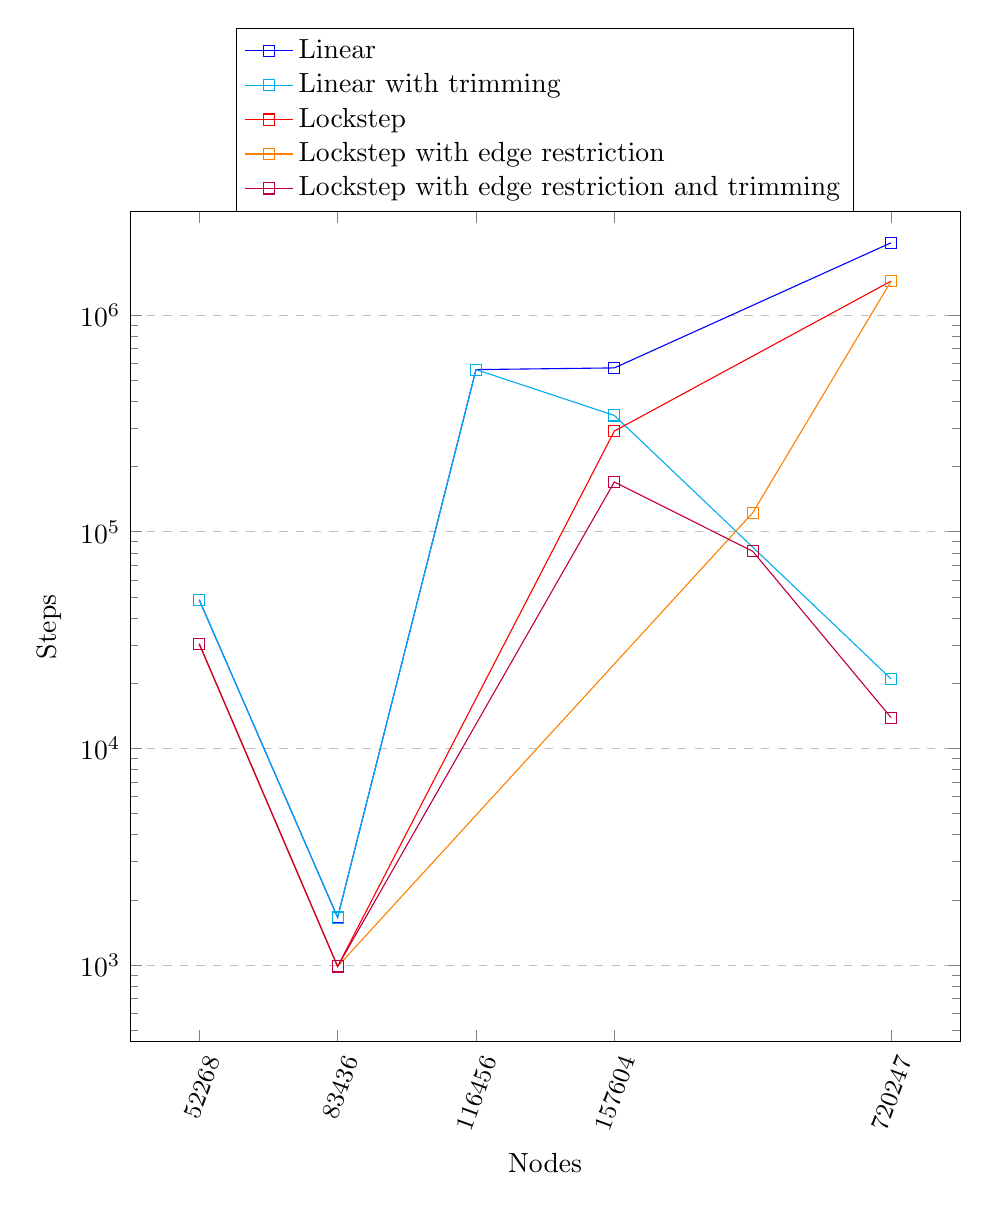
\begin{tikzpicture}
\begin{axis}[
height = \textwidth,
width=\textwidth,
xtick=data,
x tick label style = {font = \small, align = center, rotate = 70, anchor = north east},
title={Big graphs},
xlabel={Nodes},
ylabel={Steps},
ymin=0, ymax=3000000,
legend style={at={(0.5,1)},anchor=south,legend cell align=left},
ymajorgrids=true,
grid style=dashed,
ymode=log,
log basis y={10},
symbolic x coords={52268, 83436, 116456, 157604, 281903, 720247}]
\addplot[color=blue,mark=square,]coordinates {(52268, 48495)(83436, 1661)(116456, 560414)(157604, 570525)(281903, 0)(720247, 2156545)};
\addplot[color=cyan,mark=square,]coordinates {(52268, 48497)(83436, 1658)(116456, 560411)(157604, 344348)(281903, 0)(720247, 20945)};
\addplot[color=red,mark=square,]coordinates {(52268, 30384)(83436, 986)(116456, 0)(157604, 291672)(281903, 0)(720247, 1435356)};
\addplot[color=orange,mark=square,]coordinates {(52268, 30384)(83436, 986)(116456, 0)(157604, 0)(281903, 122371)(720247, 1435356)};
\addplot[color=purple,mark=square,]coordinates {(52268, 30386)(83436, 986)(116456, 0)(157604, 169828)(281903, 81275)(720247, 13872)};
\legend{Linear, Linear with trimming, Lockstep, Lockstep with edge restriction, Lockstep with edge restriction and trimming}
\end{axis}
\end{tikzpicture}

\subsection{Nodes vs. Time}

Since the first comparison didn't give us much new insight, we decided to also compare the number of nodes to the time it takes to find SCCs. This showed a stronger positive correlation. We noticed that for both small and large grpahs,  the linear-algorithm tends to take less time to run, while the Lockstep algorithm tends to jump to much higher values the more nodes there are.

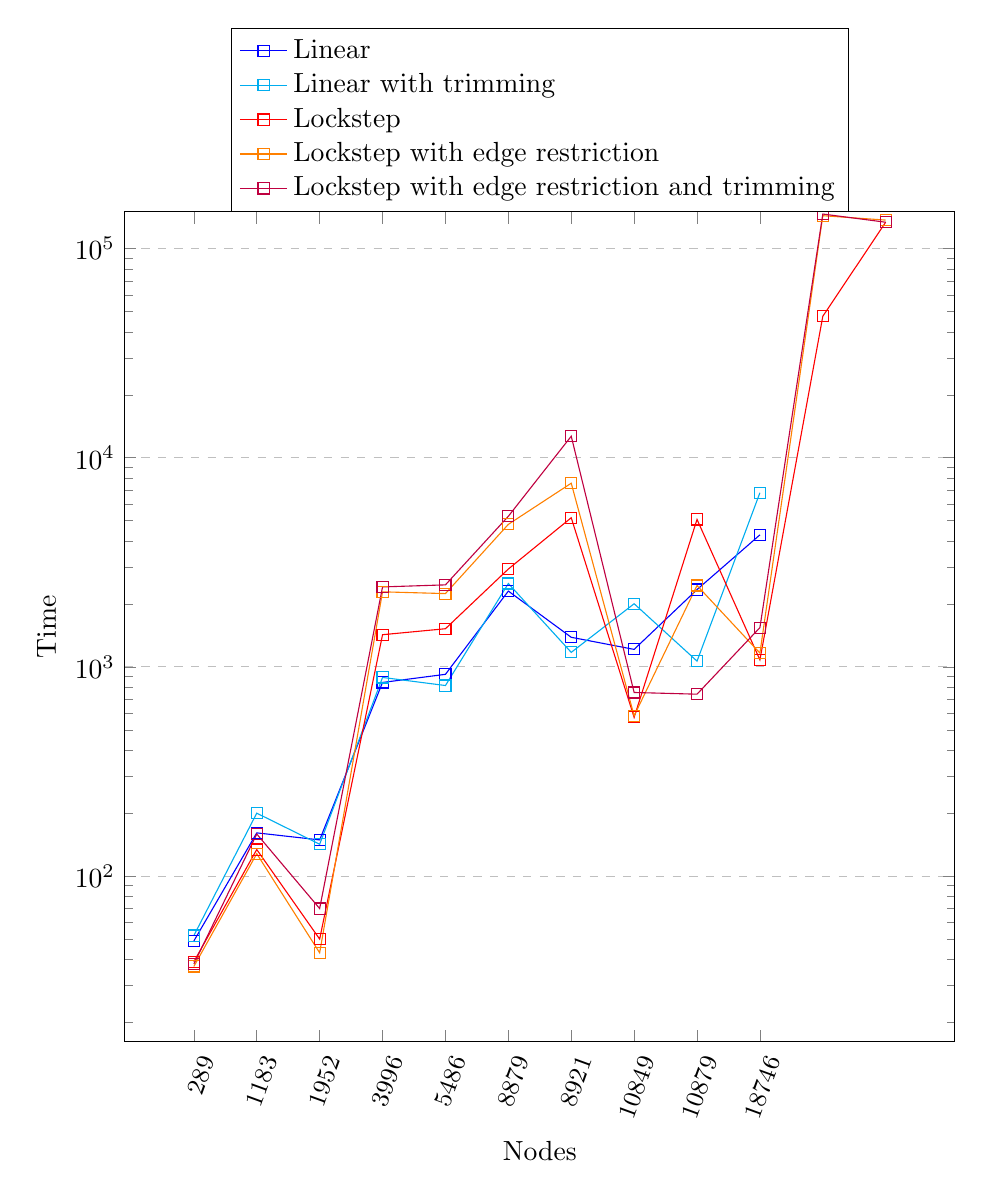
\begin{tikzpicture}
\begin{axis}[
height = \textwidth,
width=\textwidth,
xtick=data,
x tick label style = {font = \small, align = center, rotate = 70, anchor = north east},
title={Small graphs},
xlabel={Nodes},
ylabel={Time},
ymin=0, ymax=150000,
legend style={at={(0.5,1)},anchor=south,legend cell align=left},
ymajorgrids=true,
grid style=dashed,
ymode=log,
log basis y={10},
symbolic x coords={289, 1183, 1952, 3996, 5486, 8879, 8921, 10849, 10879, 18746, 25217, 40006 }]
\addplot[color=blue,mark=square,]coordinates {(289, 49)(1183, 161)(1952, 149)(3996, 843)(5486, 922)(8879, 2305)(8921, 1386)(10849, 1213)(10879, 2343)(18746, 4279)(25217, 0)(40006, 0)};
\addplot[color=cyan,mark=square,]coordinates {(289, 52)(1183, 200)(1952, 142)(3996, 891)(5486, 815)(8879, 2505)(8921, 1174)(10849, 2005)(10879, 1066)(18746, 6804)(25217, 0)(40006, 0)};
\addplot[color=red,mark=square,]coordinates {(289, 39)(1183, 134)(1952, 50)(3996, 1426)(5486, 1523)(8879, 2938)(8921, 5167)(10849, 574)(10879, 5072)(18746, 1081)(25217, 47465)(40006, 133708)};
\addplot[color=orange,mark=square,]coordinates {(289, 37)(1183, 128)(1952, 43)(3996, 2286)(5486, 2242)(8879, 4804)(8921, 7558)(10849, 584)(10879, 2451)(18746, 1165)(25217, 143599)(40006, 136794)};
\addplot[color=purple,mark=square,]coordinates {(289, 38)(1183, 159)(1952, 70)(3996, 2413)(5486, 2468)(8879, 5250)(8921, 12674)(10849, 755)(10879, 741)(18746, 1542)(25217, 146235)(40006, 133621)};
\legend{Linear, Linear with trimming, Lockstep, Lockstep with edge restriction, Lockstep with edge restriction and trimming}
\end{axis}
\end{tikzpicture}

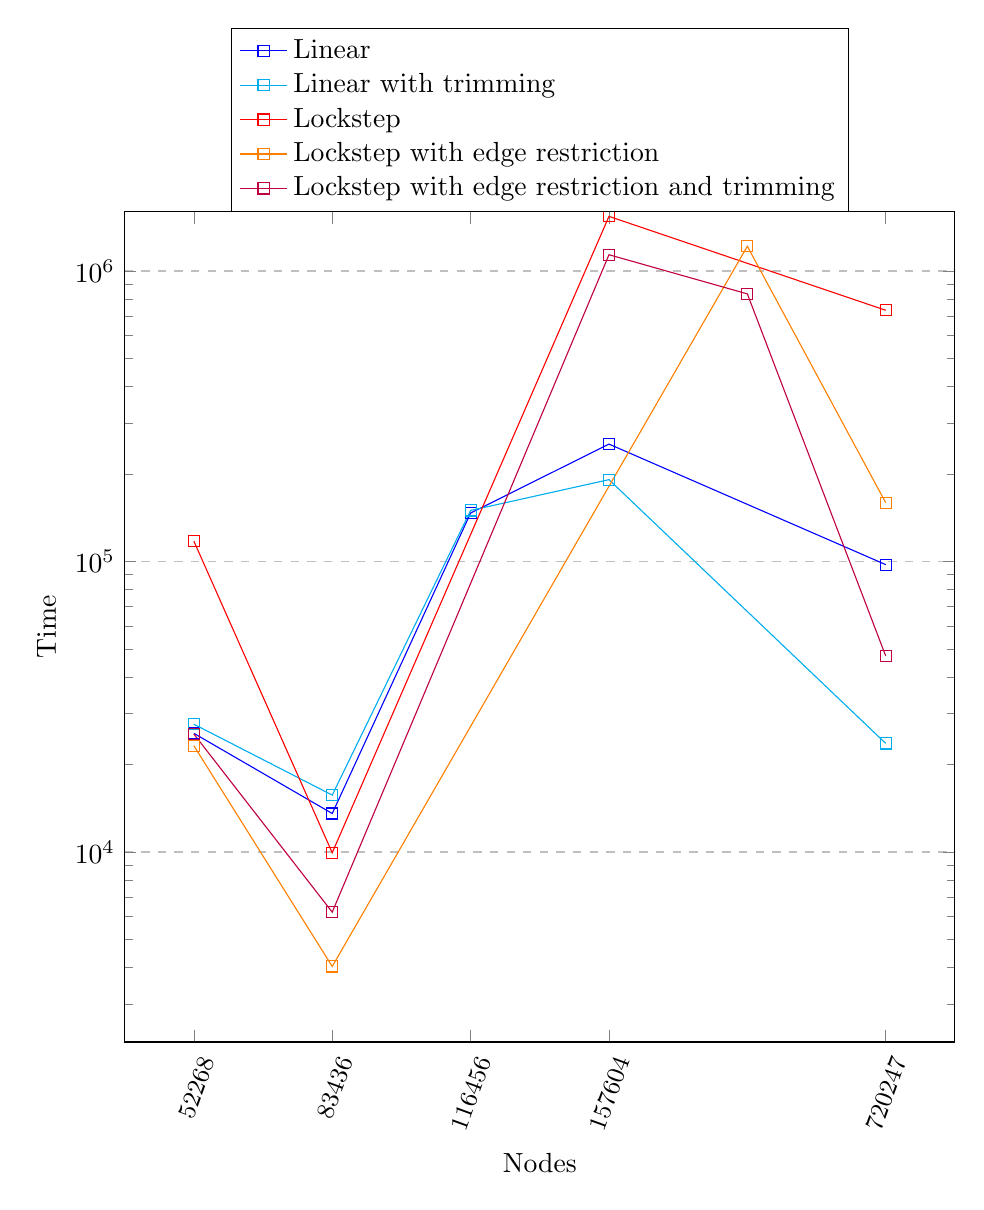
\begin{tikzpicture}
\begin{axis}[
height = \textwidth,
width=\textwidth,
xtick=data,
x tick label style = {font = \small, align = center, rotate = 70, anchor = north east},
title={Big graphs},
xlabel={Nodes},
ylabel={Time},
ymin=0, ymax=1600000,
legend style={at={(0.5,1)},anchor=south,legend cell align=left},
ymajorgrids=true,
grid style=dashed,
ymode=log,
log basis y={10},
symbolic x coords={52268, 83436, 116456, 157604, 281903, 720247 }]
\addplot[color=blue,mark=square,]coordinates {(52268, 25608)(83436, 13562)(116456, 146786)(157604, 253563)(281903, 0)(720247, 97531)};
\addplot[color=cyan,mark=square,]coordinates {(52268, 27534)(83436, 15691)(116456, 149855)(157604, 191313)(281903, 0)(720247, 23638)};
\addplot[color=red,mark=square,]coordinates {(52268, 117469)(83436, 9936)(116456, 0)(157604, 1542037)(281903, 0)(720247, 732579)};
\addplot[color=orange,mark=square,]coordinates {(52268, 23209)(83436, 4034)(116456, 0)(157604, 0)(281903, 1216873)(720247, 159329)};
\addplot[color=purple,mark=square,]coordinates {(52268, 25463)(83436, 6205)(116456, 0)(157604, 1137648)(281903, 834071)(720247, 47275)};
\legend{Linear, Linear with trimming, Lockstep, Lockstep with edge restriction, Lockstep with edge restriction and trimming}
\end{axis}
\end{tikzpicture}

\subsection{SCCs vs Steps}
The next comparison that seemed obvious to us was to compare if there was a correlation between the number of SCCs in the graph and the amount of steps it took to find them. While running some preliminary tests, we seemed to notice that the more SCCs the graph had, the longer time it would take. As can be seen in the graphs below, there is a more obvious positive correlation than there was when comparing to the number of nodes. However, there is an outlier which was a fairly large graoh with only one SCC consisting of almost all of the graph's nodes.

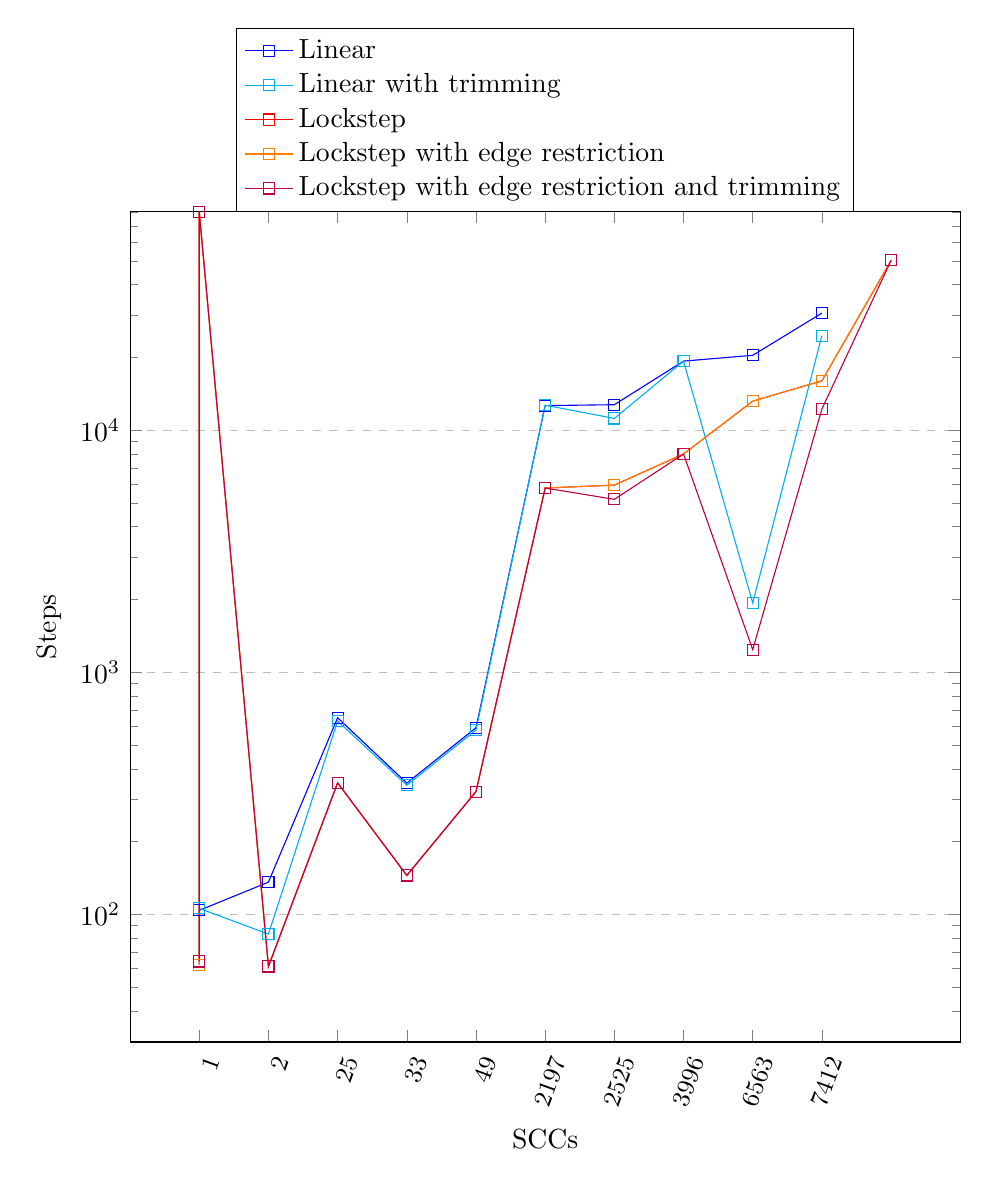
\begin{tikzpicture}
\begin{axis}[
height = \textwidth,
width=\textwidth,
xtick=data,
x tick label style = {font = \small, align = center, rotate = 70, anchor = north east},
title={Small graphs},
xlabel={SCCs},
ylabel={Steps},
ymin=0, ymax=80100,
legend style={at={(0.5,1)},anchor=south,legend cell align=left},
ymajorgrids=true,
grid style=dashed,
ymode=log,
log basis y={10},
symbolic x coords={0, 0, 1, 2, 25, 33, 49, 2197, 2525, 3996, 6563, 7412, 25217 }]
\addplot[color=blue,mark=square,]coordinates {(1, 104)(1, 0)(2, 136)(25, 650)(33, 349)(49, 591)(2197, 12664)(2525, 12773)(3996, 19344)(6563, 20434)(7412, 30529)(25217, 0)};
\addplot[color=cyan,mark=square,]coordinates {(1, 106)(1, 0)(2, 83)(25, 630)(33, 342)(49, 578)(2197, 12716)(2525, 11211)(3996, 19332)(6563, 1938)(7412, 24640)(25217, 0)};
\addplot[color=red,mark=square,]coordinates {(1, 62)(1, 80011)(2, 61)(25, 350)(33, 145)(49, 322)(2197, 5783)(2525, 5945)(3996, 7992)(6563, 13209)(7412, 16032)(25217, 50434)};
\addplot[color=orange,mark=square,]coordinates {(1, 62)(1, 80011)(2, 61)(25, 350)(33, 145)(49, 322)(2197, 5783)(2525, 5945)(3996, 7992)(6563, 13209)(7412, 16032)(25217, 50434)};
\addplot[color=purple,mark=square,]coordinates {(1, 64)(1, 80013)(2, 61)(25, 350)(33, 145)(49, 322)(2197, 5783)(2525, 5191)(3996, 7990)(6563, 1243)(7412, 12264)(25217, 50432)};
\legend{Linear, Linear with trimming, Lockstep, Lockstep with edge restriction, Lockstep with edge restriction and trimming}
\end{axis}
\end{tikzpicture}

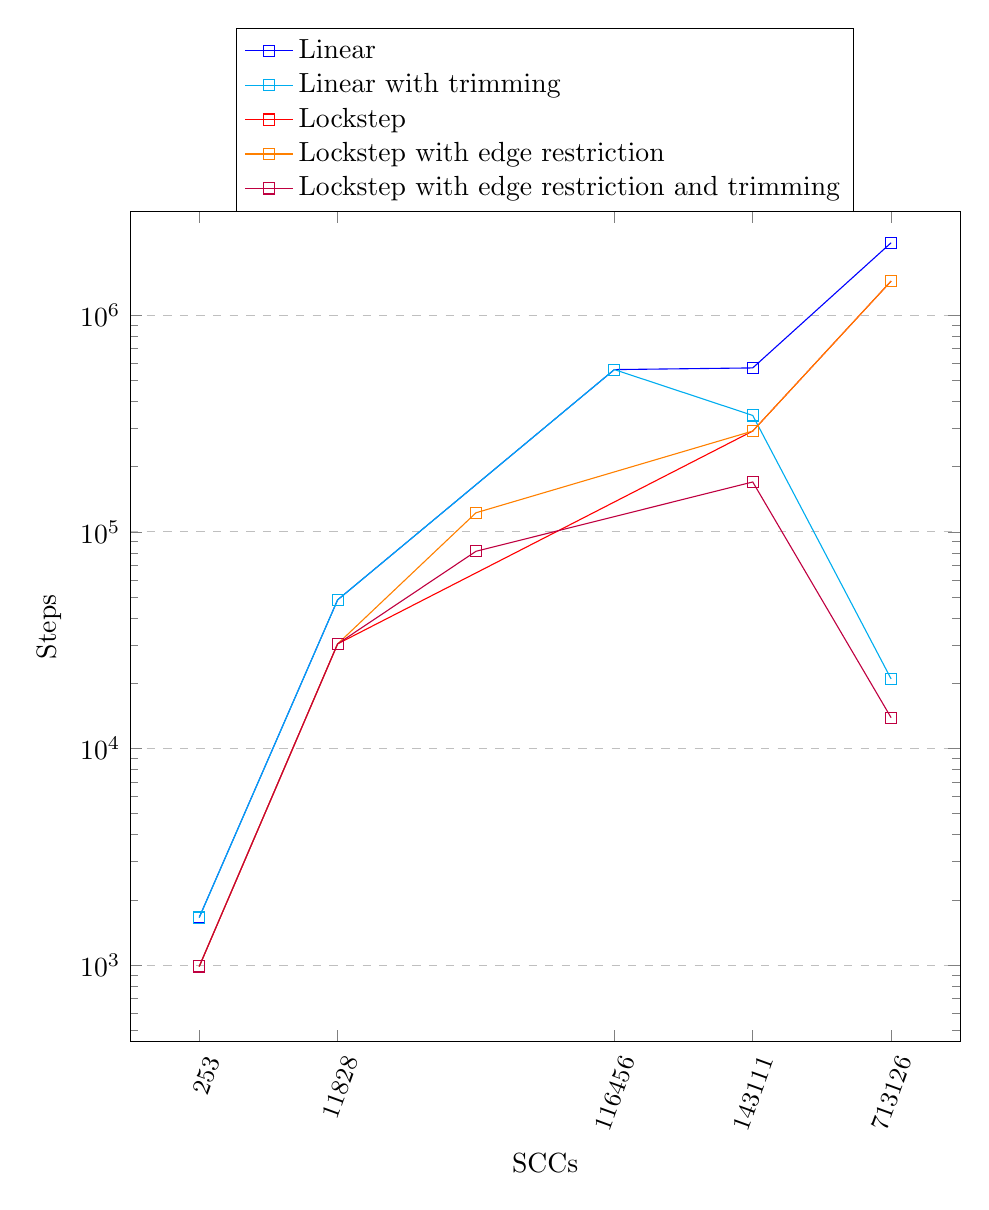
\begin{tikzpicture}
\begin{axis}[
height = \textwidth,
width=\textwidth,
xtick=data,
x tick label style = {font = \small, align = center, rotate = 70, anchor = north east},
title={Big graphs},
xlabel={SCCs},
ylabel={Steps},
ymin=0, ymax=3000000,
legend style={at={(0.5,1)},anchor=south,legend cell align=left},
ymajorgrids=true,
grid style=dashed,
ymode=log,
log basis y={10},
symbolic x coords={0, 253, 11828, 29914, 116456, 143111, 713126 }]
\addplot[color=blue,mark=square,]coordinates {(253, 1661)(11828, 48495)(29914, 0)(116456, 560414)(143111, 570525)(713126, 2156545)};
\addplot[color=cyan,mark=square,]coordinates {(253, 1658)(11828, 48497)(29914, 0)(116456, 560411)(143111, 344348)(713126, 20945)};
\addplot[color=red,mark=square,]coordinates {(253, 986)(11828, 30384)(29914, 0)(116456, 0)(143111, 291672)(713126, 1435356)};
\addplot[color=orange,mark=square,]coordinates {(253, 986)(11828, 30384)(29914, 122371)(116456, 0)(143111, 291672)(713126, 1435356)};
\addplot[color=purple,mark=square,]coordinates {(253, 986)(11828, 30386)(29914, 81275)(116456, 0)(143111, 169828)(713126, 13872)};
\legend{Linear, Linear with trimming, Lockstep, Lockstep with edge restriction, Lockstep with edge restriction and trimming}
\end{axis}
\end{tikzpicture}

\subsection{Nodes per SCC vs. Steps}
Since there was a strongly correlation between SCCs and steps then nodes and steps, we then chose to look whether the number of steps are related to the average number of nodes per SCC. The graphs below show a negative correlation between the two, with an outlier, which, as previously, only happens on the graph with one SCC containing of almost all nodes.

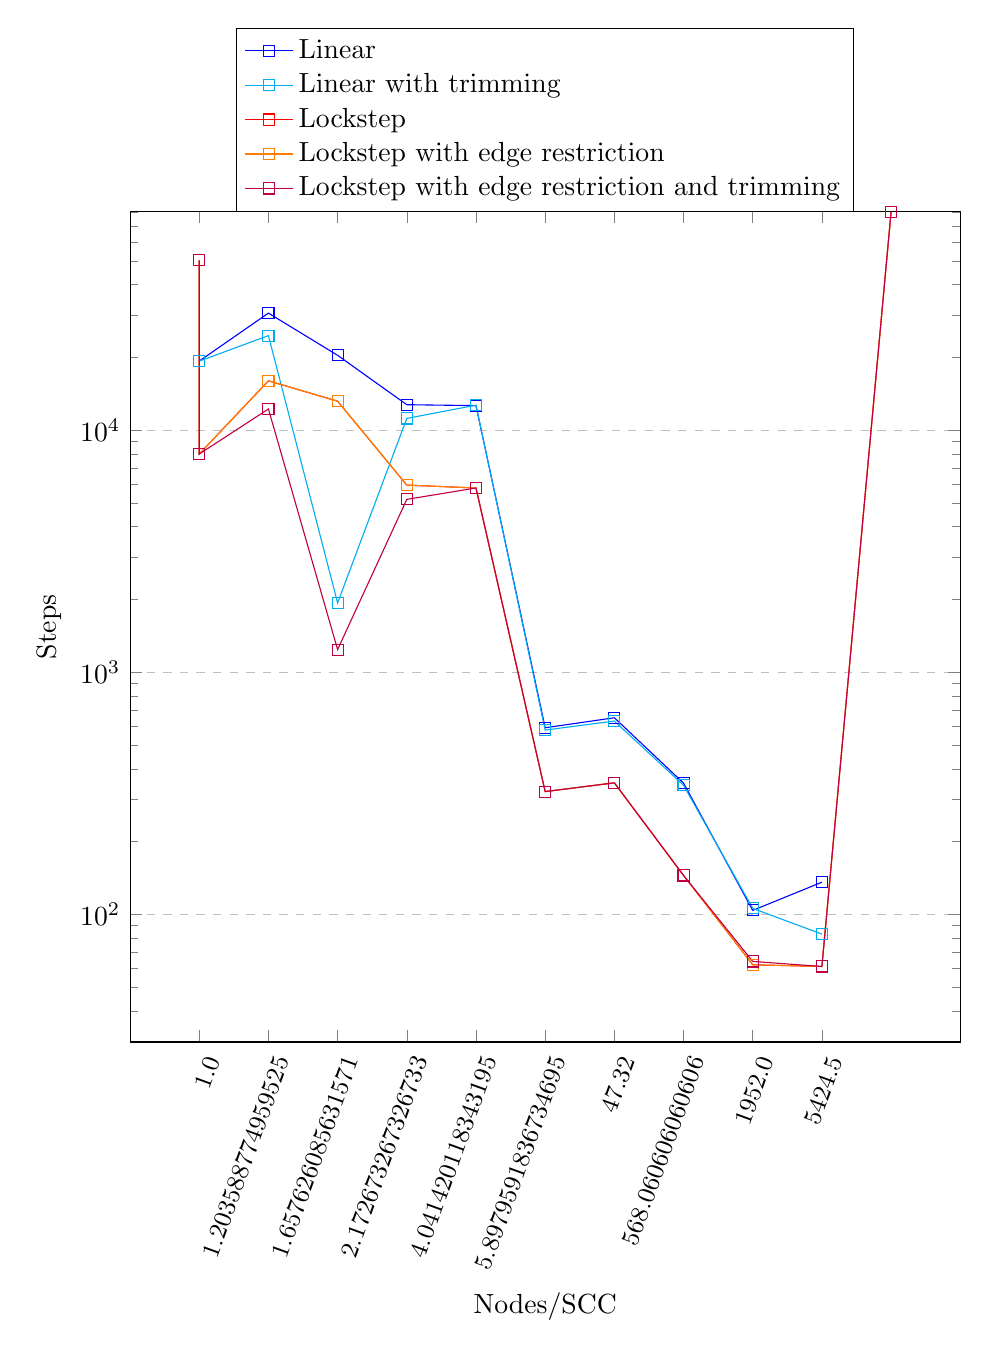
\begin{tikzpicture}
\begin{axis}[
height = \textwidth,
width=\textwidth,
xtick=data,
x tick label style = {font = \small, align = center, rotate = 70, anchor = north east},
title={Small graphs},
xlabel={Nodes/SCC},
ylabel={Steps},
ymin=0, ymax=80100,
legend style={at={(0.5,1)},anchor=south,legend cell align=left},
ymajorgrids=true,
grid style=dashed,
ymode=log,
log basis y={10},
symbolic x coords={ 1.0, 1.0, 1.203588774959525, 1.657626085631571, 2.172673267326733, 4.041420118343195, 5.8979591836734695, 47.32, 568.060606060606, 1952.0, 5424.5, 40006.0}]
\addplot[color=blue,mark=square,]coordinates {(1.0, 0)(1.0, 19344)(1.203588774959525, 30529)(1.657626085631571, 20434)(2.172673267326733, 12773)(4.041420118343195, 12664)(5.8979591836734695, 591)(47.32, 650)(568.060606060606, 349)(1952.0, 104)(5424.5, 136)(40006.0, 0)};
\addplot[color=cyan,mark=square,]coordinates {(1.0, 0)(1.0, 19332)(1.203588774959525, 24640)(1.657626085631571, 1938)(2.172673267326733, 11211)(4.041420118343195, 12716)(5.8979591836734695, 578)(47.32, 630)(568.060606060606, 342)(1952.0, 106)(5424.5, 83)(40006.0, 0)};
\addplot[color=red,mark=square,]coordinates {(1.0, 50434)(1.0, 7992)(1.203588774959525, 16032)(1.657626085631571, 13209)(2.172673267326733, 5945)(4.041420118343195, 5783)(5.8979591836734695, 322)(47.32, 350)(568.060606060606, 145)(1952.0, 62)(5424.5, 61)(40006.0, 80011)};
\addplot[color=orange,mark=square,]coordinates {(1.0, 50434)(1.0, 7992)(1.203588774959525, 16032)(1.657626085631571, 13209)(2.172673267326733, 5945)(4.041420118343195, 5783)(5.8979591836734695, 322)(47.32, 350)(568.060606060606, 145)(1952.0, 62)(5424.5, 61)(40006.0, 80011)};
\addplot[color=purple,mark=square,]coordinates {(1.0, 50432)(1.0, 7990)(1.203588774959525, 12264)(1.657626085631571, 1243)(2.172673267326733, 5191)(4.041420118343195, 5783)(5.8979591836734695, 322)(47.32, 350)(568.060606060606, 145)(1952.0, 64)(5424.5, 61)(40006.0, 80013)};
\legend{Linear, Linear with trimming, Lockstep, Lockstep with edge restriction, Lockstep with edge restriction and trimming}
\end{axis}
\end{tikzpicture}

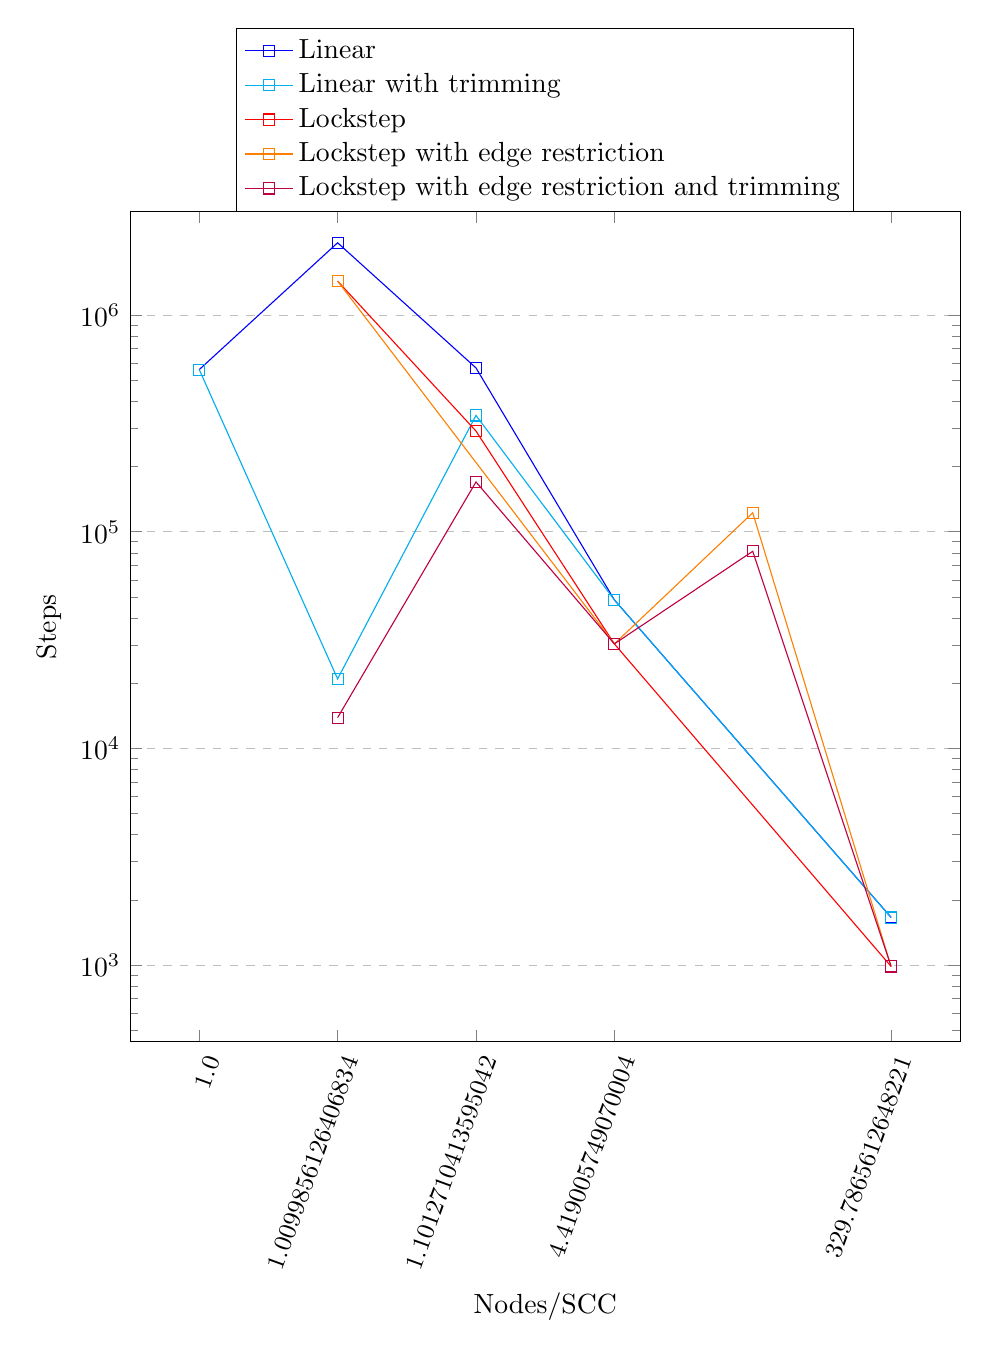
\begin{tikzpicture}
\begin{axis}[
height = \textwidth,
width=\textwidth,
xtick=data,
x tick label style = {font = \small, align = center, rotate = 70, anchor = north east},
title={Big graphs},
xlabel={Nodes/SCC},
ylabel={Steps},
ymin=0, ymax=3000000,
legend style={at={(0.5,1)},anchor=south,legend cell align=left},
ymajorgrids=true,
grid style=dashed,
ymode=log,
log basis y={10},
symbolic x coords={1.0, 1.0099856126406834, 1.1012710413595042, 4.419005749070004, 9.423781506986694, 329.7865612648221 }]
\addplot[color=blue,mark=square,]coordinates {(1.0, 560414)(1.0099856126406834, 2156545)(1.1012710413595042, 570525)(4.419005749070004, 48495)(9.423781506986694, 0)(329.7865612648221, 1661)};
\addplot[color=cyan,mark=square,]coordinates {(1.0, 560411)(1.0099856126406834, 20945)(1.1012710413595042, 344348)(4.419005749070004, 48497)(9.423781506986694, 0)(329.7865612648221, 1658)};
\addplot[color=red,mark=square,]coordinates {(1.0, 0)(1.0099856126406834, 1435356)(1.1012710413595042, 291672)(4.419005749070004, 30384)(9.423781506986694, 0)(329.7865612648221, 986)};
\addplot[color=orange,mark=square,]coordinates {(1.0, 0)(1.0099856126406834, 1435356)(4.419005749070004, 30384)(9.423781506986694, 122371)(9.423781506986694, 0)(329.7865612648221, 986)};
\addplot[color=purple,mark=square,]coordinates {(1.0, 0)(1.0099856126406834, 13872)(1.1012710413595042, 169828)(4.419005749070004, 30386)(9.423781506986694, 81275)(329.7865612648221, 986)};
\legend{Linear, Linear with trimming, Lockstep, Lockstep with edge restriction, Lockstep with edge restriction and trimming}
\end{axis}
\end{tikzpicture}

\end{document}
%%% Local Variables:
%%% mode: latex
%%% TeX-master: "../master/master"
%%% End:
